The typical approach to software application tuning begins with selecting the baseline which is a version of the application used as a reference in all the further tuning steps. The process subsequently involves profiling the application to identify the performance bottlenecks of the application.  Once identified, these bottlenecks are analyzed and a particular bottleneck is selected for tuning with the aim of improving the performance (e.g., time to solution) of the application. The tuning technique to be used on the bottleneck is identified and applied to the application and the tuning cycle begins again.

\begin{figure}[H]
\centering
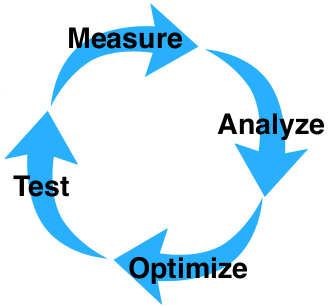
\includegraphics[scale=.6]{../BPG/images/tuning_cycle.png}
\caption{Application tuning cycle}
\label{fig:tuning_cycle}
\end{figure}

When implemented manually, the tuning process is iterative, cumbersome and often very time consuming. PTF provides tuning plugins which can perform the application tuning automatically and remove this burden of manual tuning from the application developer. The tuning plugins explore the available tuning search space, evaluate different tuning scenarios and return the end results to the users without any human interventions. Along with automatic evaluation, PTF provides smarter ways to explore possible search combinations using various search strategies. For example, in particular cases, PTF can evaluate the optimal combination without complete execution of the application which reduces the tuning times drastically. 

Use of automatic tuning contributes towards the overall productivity of software development. Additionally, due to codified expert knowledge in the form of PTF plugins it can be applied many times to different applications by users who may not be experts in application tuning.
